\chapter{Design Considerations}
\label{chap_design}

In this chapter I argue that video is the ideal storytelling medium for \textit{This Is How}. I will also iterate over the three steps of the process that were outlined in the the previous chapter and present design considerations for each with regards to video as a medium. 

\section{Choosing a medium}

\textit{This is How} is a story-centric crowdsourcing platform. Given the centrality of storytelling to the process, it’s critical to ask what medium is best for conveying these stories?

The stories presented by nonprofits in the previous chapter were told in person and in an informal manner. No structure was forced yet it did exist. It was imposed by the experience of the nonprofit in presenting their work,  a grasp of their goals and familiarity with processes. For makers, the ability to intervene and ask questions, explore and touch the surrounding, was key for a deep understanding of the organization, their challenges and constraints. 

This full sensory experience is difficult to translate into the virtual realm with today's technology. How can we create an experience that is as expressive, natural to the stakeholders, provides an understanding of the surroundings and allows for contextual discussion?

\section{Video}

Video is expressive and raw. To understand a story, it can be helpful for participants to have an unfiltered point of view. Often times the observations participants make relate to items they have seen in the surrounding and not to the main narrative the organization is trying to tell. While text often has a clearer message to it, it has already been digested to fit the narrative of the author. While the same can be said about edited video content, there is still an inherent feel of the surrounding to the medium. 

Beyond that, it is important to use a medium that users are already familiar with. Online video is extremely popular and familiar. Every minute, 500 hours worth of video are being uploaded to Youtube\cite{youtubestats}, the most popular video sharing online service. It is clear that people are capturing video. Nonprofits also already have the basic tools needed to participate: a recording device in the form of a smart-phone and in many cases broadband Internet access. 

\subsection{Limitations of Video} 

Video is far from being a perfect medium. While many nonprofit organizations might demonstrate a high level of present-ability, there is no guarantee that their ability to produce these videos will match. Creating compelling video content is difficult. A good video should strike a balance between duration and depth that makes is easy to digest yet presents enough details to get participants interested. 

The above issue is worsened by the linear nature of video, the fact that it has predetermined duration and pace makes is hard to skim over and explore. This also raises concern regarding the ability to create contextual discussion. How can we facilitate discussion over specific objects in space and time?

I'll revisit some of these issues and suggest ways to address them in the following sections.

\section{This is How}

As part of this thesis I built a web platform, \textit{This is How}, that allows nonprofits to upload a story in the form a video. This story describes the work of the organization and the processes they employ. It also allow makers to browse through these stories, engage in discussion with the organization to deepen their understanding, and finally, collaboratively brainstorm. 

In the next three subsections I drill down into the design considerations of each of the steps we outlined in Chapter 3: Discovery, Interactive Exploration and Brainstorming. These consideration include requirements, related work and my approach. 

\subsection{Discovery - Video Metadata}
In all of the cases examined in the preliminary study, discovery is one of the most challenging issues. This is How uses metadata as a driver for discovery. 

Video contains an abundance of informations: topics discussed, number of people in it, subtitles, scenery, sound track and the exact timestamps of all of the above. This data is commonly referred to as metadata. Tapping into this data and indexing it allows for searchability and semantic linking\cite{jain1994metadata}. If the topic discussed in a story is bottling milk, perhaps a juice startup can also benefit from the knowledge?

However, detailed metadata is usually not present in videos, especially not in amateur ones. In addition, it is cumbersome to manually add metadata and one cannot expect users to manually input all this information.

The solution I propose is to employ an automatic metadata generator that will work in conjunction with simple manual data input, to generate a list of tags per video. These tags will be generated according to identified entities, both through extraction of keywords from transcribed text and through image recognition techniques. The tags, for example such as \textit{Bottle} or \textit{Donation}, can be used to browse stories by a tag filter. In the future, tags can also be used create semantic links between different stories.

\subsection{Interactive Exploration - HyperMedia}

In the interactive exploration part of the process I wish to address two of the main issues related to the chosen medium of video. How to enable contextual discussion and allow for easy exploration? Following is a review of related work and a proposed approach. 

Regarding contextual discussion, Some video viewing platforms, such as Youtube, address the contextual discussion issue using hyperlinked timestamps. This means that in the regular, linear, commenting systems, users can mention timestamps. These timestamps, for example  \textit{1:20}, will automatically be hyperlink to the relevant time in the video. In the case of \textit{1:20}, clicking on it will seek the video to one minute and twenty seconds. 

   \begin{figure}[thpb]
      \centering
      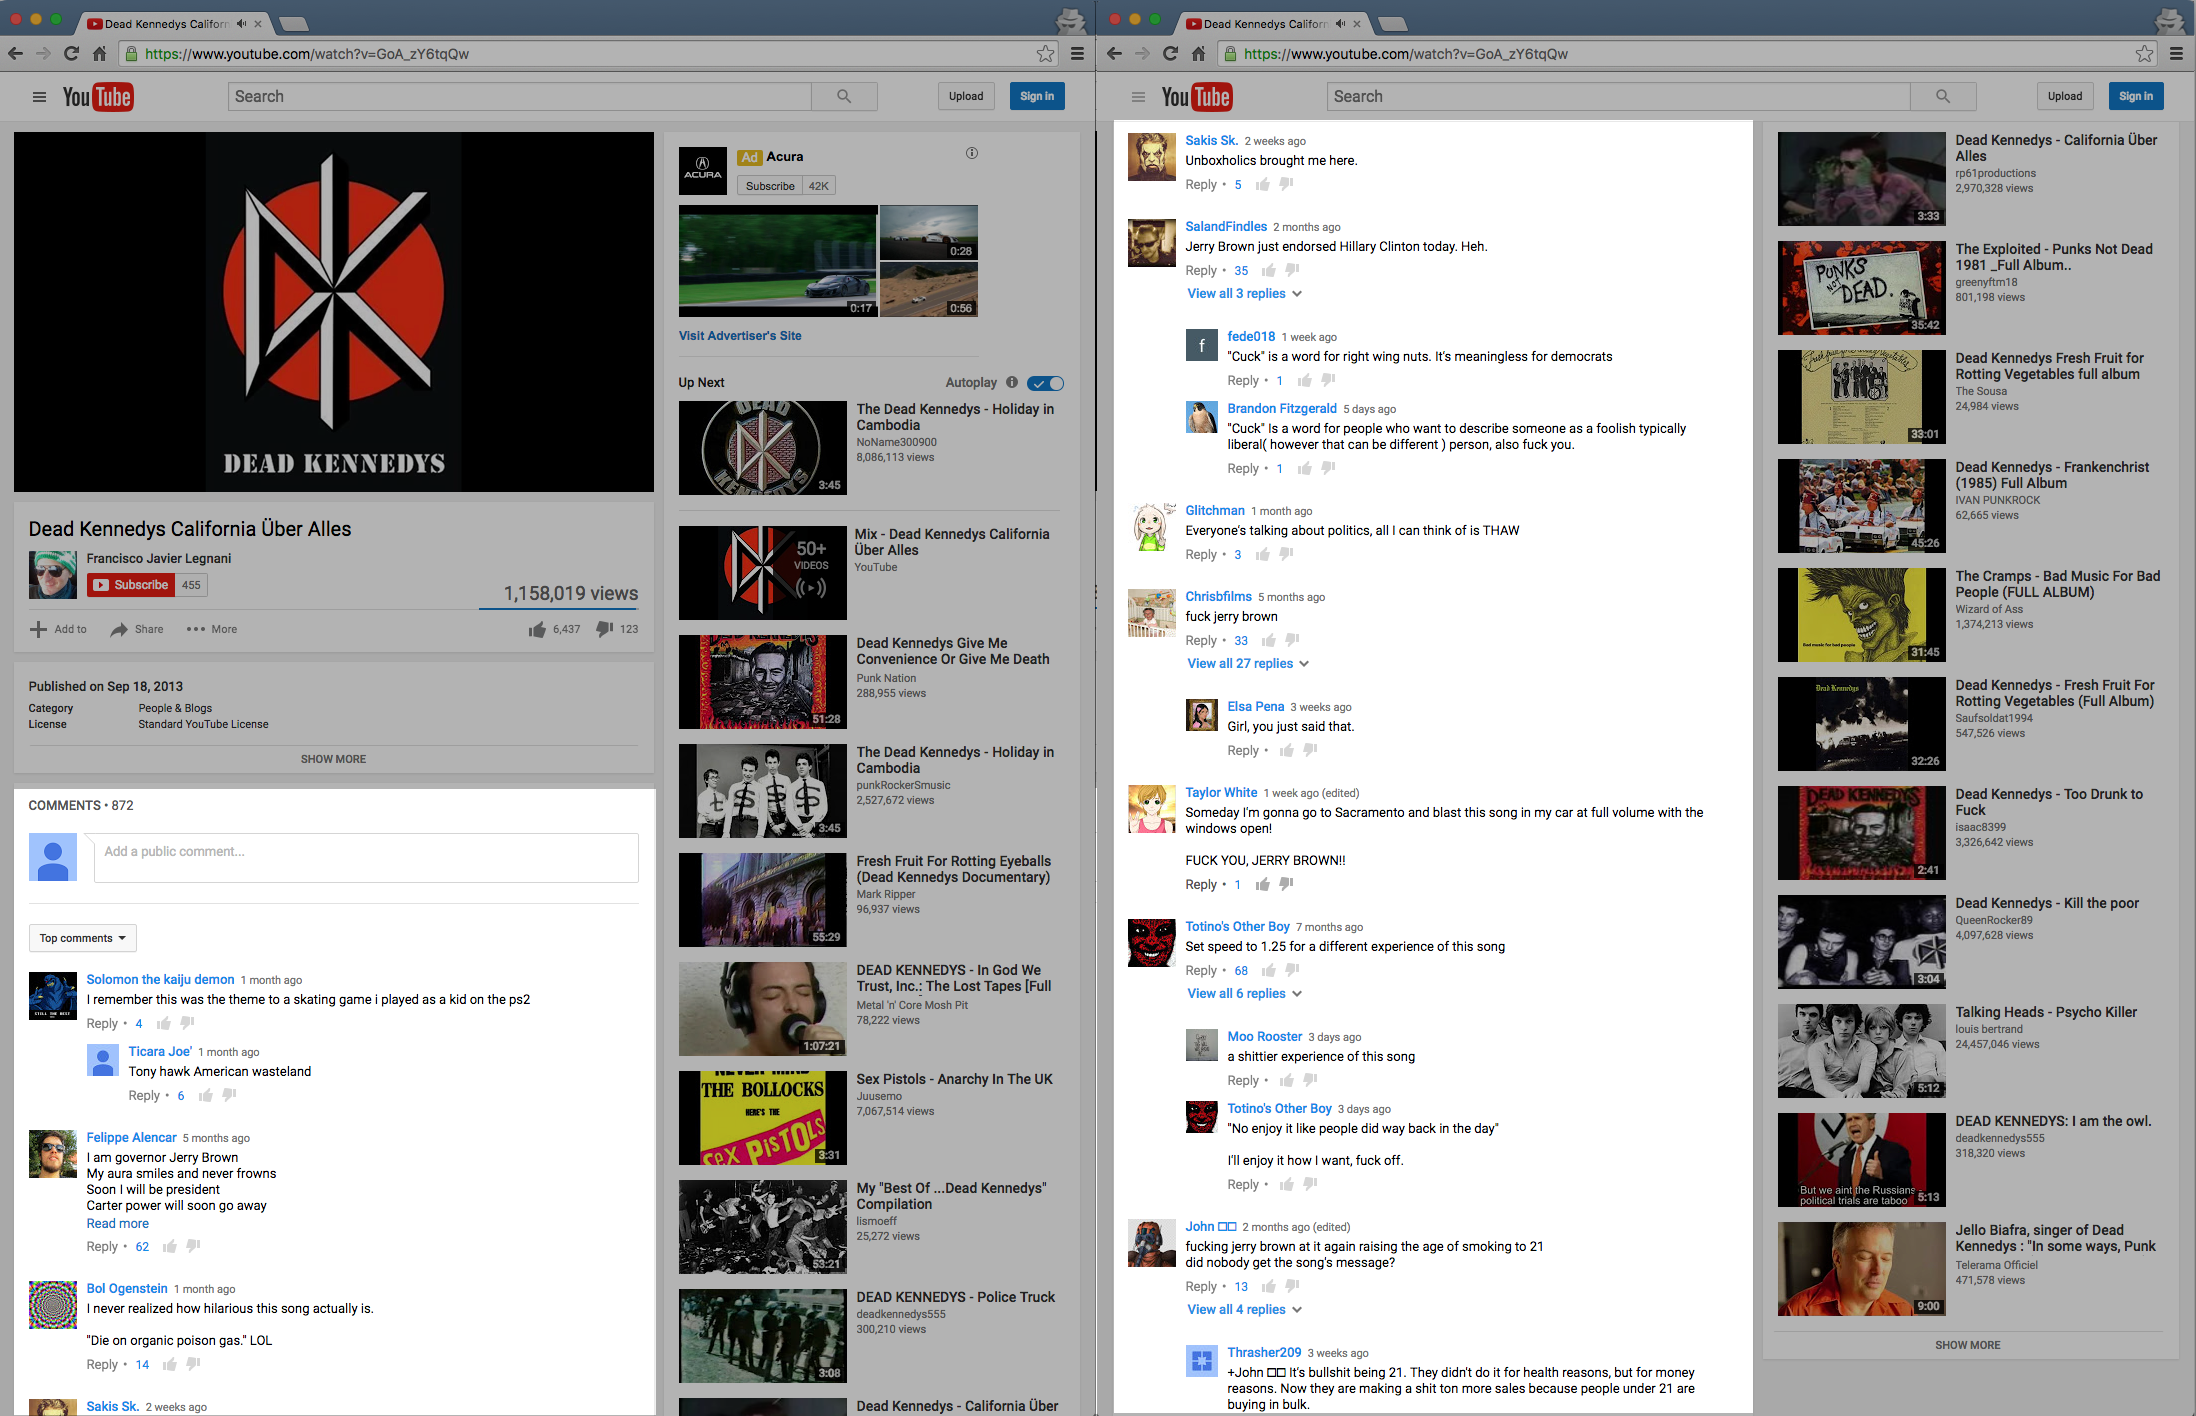
\includegraphics[width=\textwidth]{figures/youtube-left.png}
      \caption{Youtube comments. First page is on the left, second is on the right}
      \label{fig_youtube_comments}
   \end{figure}

While this does allow for the addition of time context, these comments behave just like any other. They are presented in the order in which they were inputted, there is no indicator about their existence at playtime or when clusters of them appear and they are generally second class citizens in the video playback experience

Soundcloud \cite{soundcloud}, a music streaming service, attempts to solve this issue for web-based audio streaming. Its music player interfaces place indicators of timestamped comments on the seek bar of the audio clip. The actual comment text is displayed when the playback timestamp matches that of the comment or when the listener hovers their mouse above the indicator. This approach puts comments in the front of the experience and results in clusters of indicators that immediately reveal what are the most discussed parts of the track.

   \begin{figure}[thpb]
      \centering
      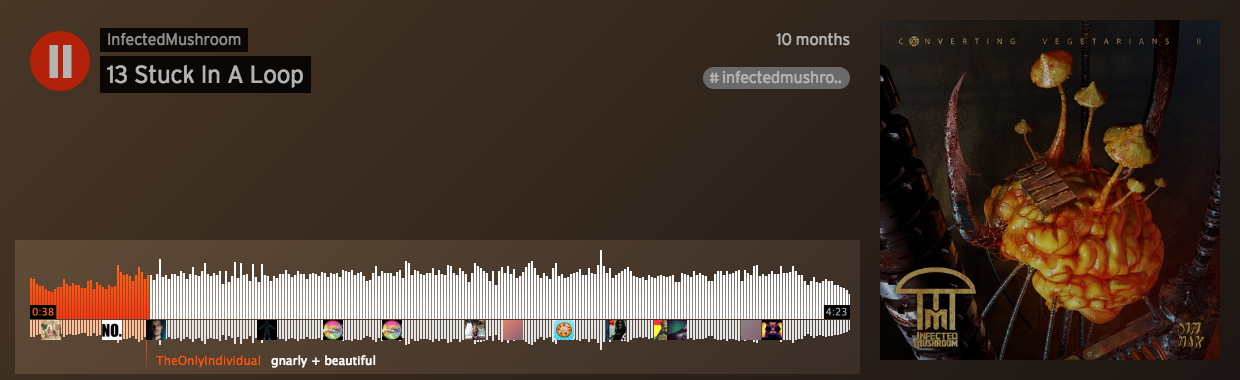
\includegraphics[width=\textwidth]{figures/soundcloud.png}
      \caption{Soundcloud comments. Indicators are embedded into the seek bar}
      \label{fig_youtube_comments}
   \end{figure}

CATool\cite{catool}, a collaborative annotation tool for video developed at Harvard, is aimed at the academic community and allows faculty and students to discuss video clips using timestamped comments and comment replies.

   \begin{figure}[thpb]
      \centering
      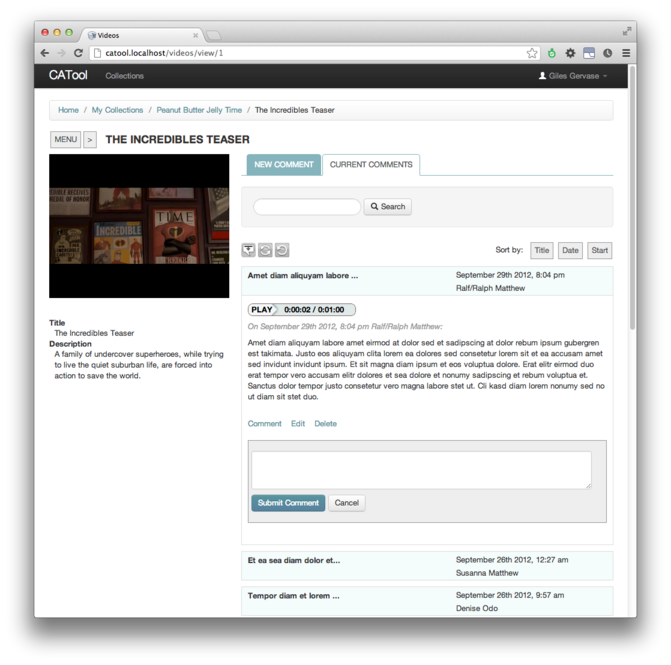
\includegraphics[width=\textwidth]{figures/catool.png}
      \caption{CATool\cite{catool} - a collaborative video annotation tool}
      \label{fig_catool}
   \end{figure}

Inspired by these platforms and by the work done in the field of hypermedia (covered in the Background Chapter), I propose a novel user interface that treats discussion as hyper layers in video. In it, Comments are: 

\begin{itemize}

\item \textit{Textual hyper layers} on top of the main story video. 

\item \textit{Timestamped} according to the playback time when they're entered and only appear in that time in the playback. 

\item \textit{Discuss-able}, each one can collapse into it's own thread that allows for further discussion, including text and video messages. 

\item \textit{Indicated} in the video seek bar according to their timestamp.

\end{itemize}

This allows participants to ask questions that relate to a specific point in time and the Organization to answer with rich media, including videos that “drill down”, providing more context in response to a question. It also allows other participants to quickly see where discussions are happening in the video and skim by navigating between them. These properties will be demonstrated in the implementation chapter.

\subsection{Brainstorming - Collaborative Pads}

As presented in the previous chapter, brainstorming takes many forms. Unlike conversations, which can be modeled as a set of messages, whether directed or broadcasted, Brainstorming also includes the concept of a shared mental model that can be collaboratively manipulated. While this model can live solely inside the head of the participants, it is not a scalable approach. Successful (capital S!) strategies include using whiteboards, sticky notes, or other tools to allow users express and share their mental models with others. How can we implement such a shared mental model for remote participants?

The usage of a networked computer as a medium that facilitates a shared mental model was first described in 1968 by J.C.R. Licklider. After first attending a meeting in which all participants had a networked computer with access to shared editable resources, Licklider concluded that ``In a few years, men will be able to communicate more effectively through a machine than face to face.''\cite{licklider1968computer}

Nowadays, a common tool to facilitate these shared mental models are real time collaborative text editors. These allow for multiple users to edit the same document at the same time while making changes visible to all other users in near real time. Most of these tools also allow for the tracking of changes, record authorship, and provide a discussion mechanism. Some notable editors in this space include Google Docs\cite{gdocs}, Apache Wave\cite{wave} and Etherpad\cite{etherpad}. 

A real time shared editor fits our needs because it provides a basis for Brainstorming without enforcing too much structure. Given that the range of topics and participants is expected to be wide, the simplicity of text provides an optimal format. 

I propose using collaborative document editing as a basis for Brainstorming. Any participant will be able to propose an idea which then turns into a collaborative text document for collaboratively shaping the idea and discussing it. In the future, these documents could also link to specific frames, comment and comment threads in the video. 